
由弗洛尔对 Arnold 猜想的证明以及随之产生的\BookRecordIndex{T0132}弗洛尔同调概念，可以得到一种与此前完全
不同的\BookRecordIndex{T0229}量子上同调研究途径（参见 \srcite{113,116}）。本章将概述辛\BookRecordIndex{T0132}弗洛尔同调的构造，但
不提供实施这一纲领所需的额外分析细节。弗洛尔最初在单调\BookRecordIndex{T0358}辛流形的背景下发展了这一同调
理论；后来 Hofer--Salamon \srcite{180} 与 Ono \srcite{313} 把它推广到\BookRecordIndex{T0058}半正情形。下面
第~\ref{sec:12-1}、\ref{sec:12-2} 与 \ref{sec:12-3} 节所解释的正是这一推广。我们还将介绍
Piunikhin--Salamon--Schwarz \srcite{323} 的构造：它给出\BookRecordIndex{T0229}量子上同调到弗洛尔上同调的
一个同构，并把\BookRecordIndex{T0228}量子杯积与弗洛尔上同调上的\BookRecordIndex{T0217}裤形乘积交织起来。

本章叙述中略去的主要技术要点有三项：第一，圆柱上弗洛尔方程解的 Fredholm 理论以及
Conley--Zehnder 指数；第二，\BookRecordIndex{T0131}弗洛尔连接轨道的\BookRecordIndex{T0166}横截性理论；第三，弗洛尔\BookRecordIndex{T0256}粘合定理。除
弗洛尔的原始论文外，证明细节还可见 Floer--Hofer--Salamon \srcite{119}、
Floer--Hofer \srcite{118}、Schwarz \srcite{358}、Salamon--Zehnder \srcite{356}、
Robbin--Salamon \srcite{335,336}、Salamon \srcite{353} 以及 Audin--Damian
\srcite{24} 的专著。与此前一样，我们不讨论 Fukaya--Ono \srcite{127} 和
Liu--Tian \srcite{249} 对一般紧\BookRecordIndex{T0358}辛流形的推广。

引入基本设置后，我们将说明\BookRecordIndex{T0132}弗洛尔同调与\BookRecordIndex{T0161}哈密顿辛微分同胚群
$\operatorname{Ham}(M,\omega)$ 的研究有何关系。第~\ref{sec:12-4} 节描述其万有覆盖
$\widetilde{\operatorname{Ham}}(M,\omega)$ 中元素的\BookRecordIndex{T0271}谱不变量。这些不变量建立在辛作用
泛函给出的弗洛尔上链复形\BookRecordIndex{T0239}滤过之上，并产生 Schwarz 与 Oh 所提出的一种有趣的 \BookRecordIndex{T0027}Hofer
度量变体。我们的叙述主要遵循 Schwarz \srcite{360} 和 Oh \srcite{306,307}。除通常的
\BookRecordIndex{T0058}半正性假设外，为简化起见还假设 $[\omega]$ 是整数类。第~\ref{sec:12-5} 节将回到 \BookRecordIndex{T0047}Seidel 表示，
用\BookRecordIndex{T0132}弗洛尔同调来表述它，并解释它对\BookRecordIndex{T0271}谱不变量的影响。

辛\BookRecordIndex{T0132}弗洛尔同调还有一个本章不讨论的版本，用来研究\BookRecordIndex{T0219}拉格朗日子流形的交。弗洛尔
\srcite{113,114} 最早在两个\BookRecordIndex{T0219}拉格朗日子流形\BookRecordIndex{T0158}哈密顿同痕且 $\pi_2(M,L)=0$ 的假设下发展了
这一理论。Oh \srcite{303} 把它推广到单调情形；此后 Fukaya--Oh--Ohta--Ono
\srcite{128} 又为拉格朗日\BookRecordIndex{T0132}弗洛尔同调发展出适用于所有紧\BookRecordIndex{T0358}辛流形的障碍理论。

Donaldson 指出，可以把\BookRecordIndex{T0132}弗洛尔同调群看作一个范畴的态射；这个范畴的对象是给定\BookRecordIndex{T0358}辛流形
$(M,\omega)$ 的\BookRecordIndex{T0219}拉格朗日子流形（相应地，也可以是辛微分同胚）。复合律由计数全纯三角形
定义，它是\BookRecordIndex{T0217}裤形乘积的类似物。Fukaya \srcite{125} 进一步发展了这一观点，并发现了链\BookRecordIndex{T0072}层次
\BookRecordIndex{T0132}弗洛尔同调背后的 $A_\infty$ 结构。

第~\ref{sec:12-6} 节将概述 Donaldson 的辛微分同胚范畴。Seidel \srcite{362} 巧妙地运用所得乘积
结构，证明了存在光滑同痕但不\BookRecordIndex{T0361}辛同痕的辛微分同胚。他发现了辛\BookRecordIndex{T0132}弗洛尔同调中的一个正合
序列，并借此完成了许多应用，其中包括计算某些辛微分同胚的\BookRecordIndex{T0132}弗洛尔同调群，从而区分它们
的\BookRecordIndex{T0361}辛同痕类。Seidel 正合序列，尤其是它与 \BookRecordIndex{T0021}Fukaya 范畴的联系，产生了许多彼此不同而又
引人注目的推论，例如关于仿射 Calabi--Yau 流形的镜像对称，以及球面余切丛中\BookRecordIndex{T0401}正合
拉格朗日子流形的拓扑。

\BookRecordIndex{T0132}弗洛尔同调还有更多版本，例如作为三维流形的不变量 \srcite{117}；它们是带边光滑
四维流形之 Donaldson 不变量的重要取值对象。在这套理论中，四维流形上的反自对偶瞬子
扮演辛弗洛尔理论里 \BookRecordIndex{T0003}$J$-全纯曲线的角色。本章不讨论这一理论，尽管它与辛\BookRecordIndex{T0132}弗洛尔同调有
一些有趣联系（见 Dostoglou--Salamon \srcite{90,91,92}）。Donaldson 的新著
\srcite{87} 是这一组思想的极佳参考。

在三、四维 Floer--Donaldson 理论中十分明显的量子场论图景，也出现在
Eliashberg--Givental--Hofer \srcite{101} 关于辛拓扑的新近工作中。他们为接触流形发展了
\BookRecordIndex{T0132}弗洛尔同调的类似物，其最简单版本称为接触同调。这些同调群是带接触边界\BookRecordIndex{T0358}辛流形的
\BookRecordIndex{T0143}格罗莫夫--威滕不变量的取值对象；沿接触边界\BookRecordIndex{T0254}粘合便得到闭\BookRecordIndex{T0358}辛流形的\BookRecordIndex{T0143}格罗莫夫--威滕不变量。
这套理论同样有涉及接触边界中 Legendrian 子流形的拉格朗日版本。这些新进展有许多有趣
应用，但详述它们远远超出本书范围。

本章最后简要讨论\BookRecordIndex{T0356}辛涡旋方程（第~\ref{sec:12-7} 节）。它们是一组关于映入带哈密顿 $G$-作用之\BookRecordIndex{T0358}辛流形
$M$ 的映射的新方程，由 Salamon \srcite{64} 和 Mundet \srcite{294,295} 各自独立发现；
在物理文献中，它们称为规范化 sigma 模型。它们推广了黎曼曲面上复线丛截面的通常涡旋
方程。在平凡情形 $G=\{1\}$，它们就退化为 \BookRecordIndex{T0003}$J$-全纯曲线；对于适当选取的（无限维）环境
流形 $M$，它们还可特化为乘积四维流形 $\Sigma\times S$ 上的反自对偶瞬子方程或
Seiberg--Witten 方程。在有限维情形，它们自然出现于辛商中 \BookRecordIndex{T0003}$J$-全纯曲线的研究。正如
第~\ref{sec:11-3} 节已经提到的，辛涡旋不变量可用于计算许多有趣\BookRecordIndex{T0358}辛流形的\BookRecordIndex{T0229}量子上同调环。

\section{弗洛尔上链复形}\label{sec:12-1}

设 $(M,\omega)$ 是\BookRecordIndex{T0058}半正\BookRecordIndex{T0358}辛流形\sourcefootnote{原书此处印作
``semipositive monotone symplectic manifold''，同时要求“\BookRecordIndex{T0058}半正”和“单调”；但本节明确
讨论从单调情形到\BookRecordIndex{T0058}半正情形的推广，且后续命题与定理仅假设\BookRecordIndex{T0058}半正，故删去多余且与语境冲突的
``monotone''。}，并设
\[
  H_t=H_{t+1}:M\longrightarrow\mathbb R
\]
是一族光滑的 $1$-周期哈密顿函数。记 $X_t:M\to TM$ 为由
\[
  \iota(X_t)\omega=dH_t
\]
定义的\BookRecordIndex{T0160}哈密顿向量场，并考虑时间依赖的哈密顿微分方程
\begin{equation}\label{eq:12-1-1}
  \dot x(t)=X_t(x(t)).
\end{equation}
式~\eqref{eq:12-1-1} 的解通过
\[
  \frac d{dt}\psi_t=X_t\circ\psi_t,
  \qquad \psi_0=\operatorname{id}_M
  \sourcefootnote{原书把流的初值印作 $\psi_0=0$；映射流的初值应为恒等映射。}
\]
生成一族辛微分同胚 $\psi_t:M\to M$。按照定义，时间一映射 $\psi=\psi_1$ 的不动点与
式~\eqref{eq:12-1-1} 的 $1$-周期解一一对应。下面说明如何把可缩的 $1$-周期解解释为
$M$ 中可缩环路空间 $\mathcal L M$ 的万有覆盖上辛作用泛函的\BookRecordIndex{T0233}临界点。

对每条可缩环路 $x:\mathbb R/\mathbb Z\to M$，存在单位圆盘
$\mathbb D=\{z\in\mathbb C\mid |z|\leq1\}$ 上的光滑映射 $u:\mathbb D\to M$，满足
$u(e^{2\pi it})=x(t)$。若两张这样的圆盘 $u_1,u_2$ 的边界和
$u_1\#(-u_2)$ 在整数同调除去挠后的空间 $H_2(M)$ 中同调于零，就称它们等价。等价的偶对
记作 $[x,u_1]\sim[x,u_2]$，并以 $\widetilde{\mathcal L M}$ 表示等价类空间；它的元素也
记为 $\widetilde x$。$\widetilde{\mathcal L M}$ 是 $\mathcal L M$ 的唯一覆盖空间，其甲板
变换群是 Hurewicz 同态 $\pi_2(M)\to H_2(M)$ 的像 $H_2^S(M)\subset H_2(M)$。记
\[
  H_2^S(M)\times\widetilde{\mathcal L M}\longrightarrow
  \widetilde{\mathcal L M},\qquad (A,\widetilde x)\longmapsto A\#\widetilde x
\]
为 $H_2^S(M)$ 的显然作用。

辛作用泛函 $\mathcal A_H:\widetilde{\mathcal L M}\to\mathbb R$ 定义为
\[
  \mathcal A_H([x,u])=-\int_{\mathbb D}u^*\omega-\int_0^1H_t(x(t))\,dt,
\]
并满足
\begin{equation}\label{eq:12-1-2}
  \mathcal A_H(A\#\widetilde x)=\mathcal A_H(\widetilde x)-\omega(A).
\end{equation}
因此，与其把它看作覆盖空间上的函数，也可把它解释为环路空间 $\mathcal L M$ 上的闭
$1$-形式；这恰是 Novikov 所研究的情形（见注~\ref{rem:11-1-6}）。

第~\ref{sec:9-1} 节已经说明，$\mathcal A_H$ 的\BookRecordIndex{T0233}临界点恰是等价类 $[x,u]$，其中
$x(t)=x(t+1)$ 是式~\eqref{eq:12-1-1} 的可缩周期解（引理~\ref{lem:9-1-8}）。用
$\widetilde{\mathcal P}(H)\subset\widetilde{\mathcal L M}$ 表示\BookRecordIndex{T0233}临界点集，用
$\mathcal P_0(H)\subset\mathcal L M$ 表示相应周期解集。\BookRecordIndex{T0132}弗洛尔同调本质上是辛作用泛函
的无限维 Morse--Novikov 理论。以下始终假设所有可缩周期解都非退化，即对每个
$x\in\mathcal P_0(H)$，$d\psi_1(x(0))$ 的所有特征值都不等于 $1$。这意味着
$\mathcal A_H$ 是 $\widetilde{\mathcal L M}$ 上的 Morse 函数，也意味
$\mathcal P_0(H)$ 是有限集。

取由 $M$ 上\BookRecordIndex{T0088}殆复结构诱导的 $\mathcal L M$ 上 $L^2$-度量，并考虑 $\mathcal A_H$ 的向下
梯度流线。它们是方程
\begin{equation}\label{eq:12-1-3}
  \partial_su+J(u)\bigl(\partial_tu-X_t(u)\bigr)=0
\end{equation}
的解 $u:\mathbb R^2\to M$，满足 $u(s,t+1)=u(s,t)$ 以及
\begin{equation}\label{eq:12-1-4}
  \lim_{s\to\pm\infty}u(s,t)=x^\pm(t),
\end{equation}
其中 $x^\pm\in\mathcal P_0(H)$。记
$\mathcal M(\widetilde x^-,\widetilde x^+;H,J)$ 为这些解中满足
$\widetilde x^-\#u=\widetilde x^+$ 的空间，也简记为
$\mathcal M(\widetilde x^-,\widetilde x^+)$。它在时间平移
$u(s,t)\mapsto u(s+s_0,t)$（$s_0\in\mathbb R$）下不变；解的等价类通常称为\BookRecordIndex{T0131}弗洛尔连接
轨道或弗洛尔轨道。每个元素都有有限能量
\begin{equation}\label{eq:12-1-5}
\begin{aligned}
  E(u)&:=\frac12\int_{-\infty}^{\infty}\int_0^1
  \bigl(|\partial_su|^2+|\partial_tu-X_t(u)|^2\bigr)\,dt\,ds\\
  &=\mathcal A_H(\widetilde x^-)-\mathcal A_H(\widetilde x^+).
\end{aligned}
\end{equation}
而且，对一般的 $H:M\times\mathbb R/\mathbb Z\to\mathbb R$，此\BookRecordIndex{T0246}模空间是有限维流形，且
\[
  \dim\mathcal M(\widetilde x^-,\widetilde x^+)
  =\mu_{\mathrm{CZ}}(\widetilde x^-)-\mu_{\mathrm{CZ}}(\widetilde x^+).
\]
这里 $\mu_{\mathrm{CZ}}:\widetilde{\mathcal P}(H)\to\mathbb Z$ 是 Conley 与 Zehnder 提出的
Maslov 指数版本。定义 $\mu_{\mathrm{CZ}}([x,u])$ 时，先平凡化圆盘 $u(\mathbb D)$ 上的
切丛，再考察沿 $x(t)$ 的线性化哈密顿流所生成的辛矩阵道路。细节见
Salamon--Zehnder \srcite{356}、Dostoglou--Salamon \srcite{91}、
Robbin--Salamon \srcite{335} 与 Salamon \srcite{353}。这里只指出
\begin{equation}\label{eq:12-1-6}
  \mu_{\mathrm{CZ}}(A\#\widetilde x)=\mu_{\mathrm{CZ}}(\widetilde x)-2c_1(A)
\end{equation}
对 $\widetilde x\in\widetilde{\mathcal P}(H)$ 与 $A\in H_2^S(M)$ 成立。此外，指数可归一化
成：若 $H_t\equiv H$ 是 $C^2$-小的 Morse 函数，$x(t)\equiv x$ 是指标为
$\operatorname{ind}_H(x)$ 的\BookRecordIndex{T0233}临界点，而 $\widetilde x=[x,u]$ 中 $u(z)\equiv x$，则
\begin{equation}\label{eq:12-1-7}
  \mu_{\mathrm{CZ}}(\widetilde x)=n-\operatorname{ind}_H(x)
  =\operatorname{ind}_{-H}(x)-n.
\end{equation}

\begin{remark}\label{rem:12-1-1}
常用的归一化有多种。这里所选归一化强调：弗洛尔上同调可视为环路空间的“中维半无限
上同调”（参见 Cohen--James--Segal \srcite{73}、Givental \srcite{146}），所以把分次
中心放在零。因此，从弗洛尔上同调到\BookRecordIndex{T0229}量子上同调的自然同构把次数提高 $n$。
\end{remark}

当 $\mu_{\mathrm{CZ}}(\widetilde x)-\mu_{\mathrm{CZ}}(\widetilde y)=1$ 时，
$\mathcal M(\widetilde x,\widetilde y)$ 是一维流形，故商空间
$\mathcal M(\widetilde x,\widetilde y)/\mathbb R$ 的每一点都是孤立的。对一般的 $H$ 还有：

\begin{proposition}\label{prop:12-1-2}
设 $(M,\omega)$ \BookRecordIndex{T0058}半正。则对一般的\BookRecordIndex{T0088}殆复结构 $J$ 与一般的哈密顿量 $H$，任给
$\widetilde x,\widetilde y\in\widetilde{\mathcal P}(H)$ 满足
$\mu_{\mathrm{CZ}}(\widetilde x)-\mu_{\mathrm{CZ}}(\widetilde y)=1$，以及任意常数 $c$，都有
\[
  \sum_{\substack{\omega(A)\leq c\\c_1(A)=0}}
  \#\frac{\mathcal M(\widetilde x,A\#\widetilde y)}{\mathbb R}<\infty.
\]
\end{proposition}

这里对 $J$ 的条件是：所有单 $J$-全纯球面 $v:S^2\to M$ 都正则，即\BookRecordIndex{T0346}线性化算子 $D_v$
满射。对 $H$ 的条件是：\BookRecordIndex{T0131}弗洛尔连接轨道的\BookRecordIndex{T0346}线性化算子满射（即辛作用泛函
$\mathcal A_H$ 为 Morse--Smale），并且对所有
$\widetilde x,\widetilde y\in\widetilde{\mathcal P}(H)$ 与 $A\in H_2^S(M)$，\BookRecordIndex{T0283}求值映射
\[
\begin{split}
  &\mathcal M(\widetilde x,\widetilde y;J,H)\times S^1
  \times\mathcal M(A;J)\times_GS^2\longrightarrow M\times M,\\
  &(u,t,[v,z])\longmapsto(u(0,t),v(z))
\end{split}
\]
横截于对角线。

为证明命题~\ref{prop:12-1-2}，须证明有关\BookRecordIndex{T0246}模空间紧；若没有\BookRecordIndex{T0243}冒泡，\BookRecordIndex{T0192}紧性便成立。关键观察是：
对一般的 $J$，位于 Chern 数为零的 $J$-全纯球面上的点在 $M$ 中构成余维四的集合；因此
对一般的 $H$，这样的球面不会与孤立连接轨道相交。由 弗洛尔--\BookRecordIndex{T0139}格罗莫夫紧性，它们不可能
冒出。\BookRecordIndex{T0058}半正性又排除了负 Chern 数的 $J$-全纯球面。Chern 数至少为一的球面也不能冒出，
否则极限中会出现指标差为负的连接轨道，而一般情形下不存在这种轨道。这就是命题证明的
要点，细节见 Hofer--Salamon \srcite{180}。

每当 $\mu_{\mathrm{CZ}}(\widetilde x)-\mu_{\mathrm{CZ}}(\widetilde y)=1$，记
\[
  n(\widetilde x,\widetilde y):=
  \#\frac{\mathcal M(\widetilde x,\widetilde y)}{\mathbb R},
\]
其中连接轨道须按 Floer--Hofer \srcite{118} 中连接轨道\BookRecordIndex{T0246}模空间的一套协调定向所确定的适当
符号计数。这些数决定一个弗洛尔上链复形，现说明如下。

与\BookRecordIndex{T0229}量子上同调一样，系数环有许多选择。为简单起见，只取 Novikov 环 $\Lambda_\omega$
为系数。这里稍微修改例~\ref{ex:11-1-4}(iii) 的 $\Lambda_\omega$ 定义，只允许球面同调类。
固定带幺交换环 $R$，令 $\Lambda_\omega$ 为所有满足有限性条件
\[
  \#\{A\in H_2^S(M)\mid \lambda(A)\neq0,\ \omega(A)\leq c\}<\infty
\]
（对每个 $c\in\mathbb R$）的函数 $\lambda:H_2^S(M)\to R$ 之集。如例~\ref{ex:11-1-4}
所述，这是一个 $2\mathbb Z$-分次交换环与 $R$-模，分次由 $\deg(A):=2c_1(A)$ 给出。

定义弗洛尔上链群 $\operatorname{CF}^*:=\operatorname{CF}^*(H)$ 为所有函数
$\xi:\widetilde{\mathcal P}(H)\to R$ 之集，要求对每个 $c\in\mathbb R$ 都满足
\begin{equation}\label{eq:12-1-8}
  \#\{\widetilde x\in\widetilde{\mathcal P}(H)
  \mid \xi(\widetilde x)\neq0,\ \mathcal A_H(\widetilde x)\leq c\}<\infty.
\end{equation}
它是 Novikov 环 $\Lambda_\omega$ 上的模，其作用为
\[
  (\lambda*\xi)(\widetilde x):=\sum_A\lambda(A)\xi(A\#\widetilde x).
\]
分次定义为 $\deg(\widetilde x):=\mu_{\mathrm{CZ}}(\widetilde x)$；次数 $k$ 部分
$\operatorname{CF}^k$ 由仅在 $\mu_{\mathrm{CZ}}(\widetilde x)=k$ 的元素上非零的
$\xi\in\operatorname{CF}^*$ 构成。因此，除非 $\lambda$ 只在 $c_1(A)=0$ 时才可能非零，
作用 $\xi\mapsto\lambda*\xi$ 会改变次数。注意，$\operatorname{CF}^*(H)$ 作为
$\Lambda_\omega$-模的维数恰是哈密顿系统~\eqref{eq:12-1-1} 的可缩周期解数
$\#\mathcal P_0(H)$。事实上，此复形同构于由 $\Lambda$-模同态
$\xi:\widetilde{\mathcal P}(H)\to\Lambda$ 构成的上链复形；见注~\ref{rem:12-5-5}。

上述数 $n(\widetilde x,\widetilde y)$ 决定上边缘算子
$\delta:\operatorname{CF}^*(H)\to\operatorname{CF}^*(H)$，定义为
\begin{equation}\label{eq:12-1-9}
  (\delta\xi)(\widetilde x)=
  \sum_{\mu_{\mathrm{CZ}}(\widetilde y)=\mu_{\mathrm{CZ}}(\widetilde x)-1}
  n(\widetilde x,\widetilde y)\xi(\widetilde y).
\end{equation}
命题~\ref{prop:12-1-2} 与式~\eqref{eq:12-1-2} 保证右端对每个 $\widetilde x$ 都是
有限和，并且每个 $\xi\in\operatorname{CF}^*$ 都有
$\delta\xi\in\operatorname{CF}^*$。若 $\xi\in\operatorname{CF}^k$，则
$\delta\xi\in\operatorname{CF}^{k+1}$。

Floer \srcite{116} 在单调情形证明了 $\delta^2=0$（另见 McDuff \srcite{255} 与
Salamon--Zehnder \srcite{356}）。算子 $\delta\circ\delta$ 的系数计数从
$\widetilde x$ 到 $\widetilde y$ 的连接轨道偶对，其中 $\widetilde y$ 的指标比
$\widetilde x$ 小二。此时轨道\BookRecordIndex{T0246}模空间 $\mathcal M(\widetilde x,\widetilde y)$ 是二维的；
除去时间平移后，它形成一维定向流形，其边界正是 $\delta\circ\delta$ 所计数的那些偶对。
反过来，\BookRecordIndex{T0254}粘合构造说明每个这样的偶对都是 $\mathcal M(\widetilde x,\widetilde y)$ 某个分支
的边界。因此这些对象成对抵消，故 $\delta\circ\delta=0$。在单调情形这一论证成立，
因为任何\BookRecordIndex{T0243}冒泡都会产生负指标的\BookRecordIndex{T0131}弗洛尔连接轨道，而\BookRecordIndex{T0166}横截性排除了这种轨道。

要把论证推广到\BookRecordIndex{T0058}半正流形，必须检查\BookRecordIndex{T0243}冒泡不会造成干扰，例如不会使一维流形
$\mathcal M(\widetilde x,\widetilde y)/\mathbb R$ 出现连接轨道偶对以外的边界分支。
关键观察是：指标差为二的单参数连接轨道族仍避开 Chern 数为零的 $J$-全纯球面，因为这些
轨道在 $M$ 中构成三维集合，而那些球面构成余维四的集合。同样，Chern 数为一的全纯球面
只有与某条周期解相交时才可能冒出；对一般的 $H$ 这不会发生，因为这些球面上的点在 $M$
中构成余维二集合，而周期轨道构成一维集合。若 Chern 数至少为二的 $J$-全纯球面冒出，
它就必须附着在指标至多为零的连接轨道上；一般偶对 $(H,J)$ 不存在这种轨道，因为连接轨道
在一维时间平移下不变。因此，指标差为二的连接轨道不会\BookRecordIndex{T0243}冒泡，只能退化为两条指标差各为一
的轨道。与上述标准理论相同，这就证明 $\delta\circ\delta=0$。

故式~\eqref{eq:12-1-3} 的解决定上链复形 $(\operatorname{CF}^*,\delta)$，其同调群
\[
  \operatorname{HF}^*(H,J):=\operatorname{HF}^*(M,\omega,H,J)
  :=\frac{\ker\delta}{\operatorname{im}\delta}
\]
称为偶对 $(H,J)$ 的弗洛尔上同调群。由于上边缘映射在 $\Lambda_\omega$ 上线性，
弗洛尔上同调群构成 $\Lambda_\omega$-模。

下一个定理断言，弗洛尔上同调群与定义它时所用的\BookRecordIndex{T0088}殆复结构 $J$ 和哈密顿量 $H$ 无关。

\begin{theorem}\label{thm:12-1-3}
设 $(M,\omega)$ \BookRecordIndex{T0058}半正。若偶对 $(H^\alpha,J^\alpha)$ 与 $(H^\beta,J^\beta)$ 满足定义弗洛尔
上同调所需的\BookRecordIndex{T0408}正则性条件，则有自然同构
\[
  \Phi^{\alpha\beta}:\operatorname{HF}^*(M,\omega,H^\beta,J^\beta)
  \longrightarrow\operatorname{HF}^*(M,\omega,H^\alpha,J^\alpha).
\]
若 $(H^\gamma,J^\gamma)$ 是另一个这样的偶对，则
\[
  \Phi^{\alpha\gamma}=\Phi^{\alpha\beta}\circ\Phi^{\beta\gamma},
  \qquad \Phi^{\alpha\alpha}=\operatorname{id}.
\]
这些同构在 $\Lambda_\omega$ 上线性。
\end{theorem}

同构 $\Phi^{\alpha\beta}$ 称为\BookRecordIndex{T0133}弗洛尔延拓映射。为证明定理，选取从
$(H^\alpha,J^\alpha)$ 到 $(H^\beta,J^\beta)$ 的同伦 $(H_s,J_s)$，即当 $s$ 接近
$-\infty$ 时它等于前者，接近 $+\infty$ 时等于后者。再考虑方程~\eqref{eq:12-1-3}
的如下时间依赖版本之有限能量解：
\begin{equation}\label{eq:12-1-10}
  \partial_su+J_s(u)\bigl(\partial_tu-X_{s,t}(u)\bigr)=0,
\end{equation}
其中 $X_{s,t}\in\operatorname{Vect}(M)$ 由 $\iota(X_{s,t})\omega=dH_{s,t}$ 定义。
这里 $u$ 满足通常的周期条件 $u(s,t+1)=u(s,t)$。每个这样的解都有极限
\[
  \lim_{s\to-\infty}u(s,t)=x^\alpha(t),\qquad
  \lim_{s\to+\infty}u(s,t)=x^\beta(t),
\]
其中 $x^\alpha\in\mathcal P_0(H^\alpha)$、$x^\beta\in\mathcal P_0(H^\beta)$。取由延拓解
$u$ 拼接两端帽盘所确定的\BookRecordIndex{T0348}相容提升 $\widetilde x^\alpha$、$\widetilde x^\beta$
\sourcefootnote{原书在\BookRecordIndex{T0249}能量恒等式中省略了波浪号及帽盘数据；但辛作用泛函只定义在带帽轨道的
覆盖空间上，而两端提升的\BookRecordIndex{T0348}相容性由延拓解 $u$ 拼接帽盘确定。}。关键是
\BookRecordIndex{T0249}能量恒等式
\begin{equation}\label{eq:12-1-11}
\begin{aligned}
  E(u)&:=\int_{-\infty}^{\infty}\int_0^1|\partial_su|^2\,dt\,ds\\
  &=\mathcal A_{H^\alpha}(\widetilde x^\alpha)
  -\mathcal A_{H^\beta}(\widetilde x^\beta)
  -\int_{-\infty}^{\infty}\int_0^1(\partial_sH_{s,t})(u)\,dt\,ds.
\end{aligned}
\end{equation}
通常的\BookRecordIndex{T0192}紧性与\BookRecordIndex{T0166}横截性论证由此表明，式~\eqref{eq:12-1-10} 的解决定次数为零的链映射
$\operatorname{CF}^*(H^\beta)\to\operatorname{CF}^*(H^\alpha)$；再选同伦之间的同伦，
即可看出它在弗洛尔上同调上诱导的映射与同伦选择无关。这些论证与 Floer
\srcite{116} 在单调情形的原证明完全相同；当前情形见 Hofer--Salamon \srcite{180}。
（在 $H_2^S(M)$ 上 $c_1=[\omega]=0$ 的情形另见 Salamon--Zehnder \srcite{356}。）

\paragraph{计算弗洛尔上同调。}
依循弗洛尔的思想，可以把哈密顿量特化为一个与时间无关且 $C^2$-小的函数，并尝试证明
弗洛尔方程的相关解也与 $t$ 无关。于是弗洛尔上同调群自然同构于底流形 $M$ 取 Novikov
环 $\Lambda_\omega$ 系数的通常上同调，而后者恰是 $M$ 的\BookRecordIndex{T0229}量子上同调。为避免挠的问题，
取底环 $R$ 为 $\mathbb Q$、$\mathbb R$ 或 $\mathbb C$。尽管以下多数结果对任意底环仍然
成立，这里仍限于特征零域上的系数，以便与第~\ref{sec:11-1} 节把上同调除以挠子模的\BookRecordIndex{T0229}量子
上同调做法一致。

以下定理在单调情形由 Floer \srcite{116} 证明；当所有 $A\in\pi_2(M)$ 都满足
$c_1(A)=0$，或最小 Chern 数 $N\geq n$ 时，由 Hofer--Salamon \srcite{180} 证明。
一般情形由 Piunikhin--Salamon--Schwarz \srcite{323} 与 Liu--Tian \srcite{250} 以
不同方法处理。

\begin{theorem}\label{thm:12-1-4}
设 $(M,\omega)$ \BookRecordIndex{T0058}半正。对每个正则偶对 $(H^\alpha,J^\alpha)$，存在次数为 $n$ 的同构
\[
  \Phi^\alpha:\operatorname{HF}^*(M,\omega,H^\alpha,J^\alpha)
  \longrightarrow\operatorname{QH}^*(M;\Lambda_\omega).
\]
这些映射在如下意义下是自然的：
\[
  \Phi^\alpha\circ\Phi^{\alpha\beta}=\Phi^\beta,
\]
且它们在 $\Lambda_\omega$ 上线性。
\end{theorem}

由于稍后就会明白的理由，把此定理证明中构造的同构 $\Phi^\alpha$ 称为 PSS 映射；为清楚
起见，有时记作 $\Phi^*_{\mathrm{PSS}}$。

弗洛尔在单调情形的原证明，以及 Hofer--Salamon \srcite{180} 在\BookRecordIndex{T0058}半正情形的证明，都基于
如下思想。取 Morse 函数 $f:M\to\mathbb R$，使它关于度量
$\omega(\,\cdot\,,J\,\cdot\,)$ 的负梯度流为 Morse--Smale，并考虑与时间无关（或称自治）的哈密顿量
\[
  H_t:=-\varepsilon f,\qquad t\in\mathbb R.
\]
若 $\varepsilon$ 充分小，则式~\eqref{eq:12-1-1} 的 $1$-周期解恰为 $f$ 的\BookRecordIndex{T0233}临界点，即
$\mathcal P_0(H)=\operatorname{Crit}(f)$；由式~\eqref{eq:12-1-7}，Conley--Zehnder 指数与
Morse 指数的关系为
\[
  \mu_{\mathrm{CZ}}([x,u_x])=\operatorname{ind}_f(x)-n,
\]
其中 $u_x:\mathbb D\to M$ 是常值映射 $u_x(z)\equiv x$。函数 $f$ 的梯度流线
$u:\mathbb R\to M$ 满足常微分方程
\begin{equation}\label{eq:12-1-12}
  \dot u(s)+\nabla f(u(s))=0,
\end{equation}
它们也是偏微分方程~\eqref{eq:12-1-3} 中与 $t$ 无关的特殊解。这些解决定
\BookRecordIndex{T0037}Morse--Witten 上边缘算子
\[
  \delta_{\mathrm{MW}}:\operatorname{CM}^*(f;\Lambda_\omega)
  \longrightarrow\operatorname{CM}^*(f;\Lambda_\omega).
\]
此算子与弗洛尔上边缘 $\delta$ 定义在同一个上链复形上；由式~\eqref{eq:12-1-7}，两种
理论的上链复形分次相差 $n$。

更准确地说，上链复形 $\operatorname{CM}^*(f;\Lambda_\omega)$ 可认作所有满足下列有限性
条件的函数 $\xi:\operatorname{Crit}(f)\times H_2^S(M)\to R$ 所成的分次
$\Lambda_\omega$-模：
\begin{equation}\label{eq:12-1-13}
  \#\{(x,A)\mid \xi(x,A)\neq0,\ \omega(A)\geq c\}<\infty
\end{equation}
对每个 $c\in\mathbb R$ 成立。\footnote{当 $H_t=-f$ 时，
$\widetilde{\mathcal P}(H)$ 可与 $\operatorname{Crit}(f)\times H_2^S(M)$ 等同。在此对应下，
辛作用量是函数 $\mathcal A_f:\operatorname{Crit}(f)\times H_2^S(M)\to\mathbb R$，
$\mathcal A_f(x,A):=f(x)-\omega(A)$。因此，式~\eqref{eq:12-1-13} 的有限性条件等价于
$H_t=-f$ 时 $\operatorname{CF}^*(H)$ 定义中的有限性条件。}其 $\Lambda_\omega$-模结构由
\[
  (\lambda*\xi)(x,A):=\sum_B\lambda(B)\xi(x,A+B)
\]
给出，分次为 $\deg(x,A):=\operatorname{ind}_f(x)-2c_1(A)$，而上边缘算子为
\[
  (\delta_{\mathrm{MW}}\xi)(x,A):=\sum_y n_f(x,y)\xi(y,A).
\]
这里 $n_f(x,y)$ 是从 $x$ 到 $y$ 的连接轨道数，即式~\eqref{eq:12-1-12} 中满足
\[
  \lim_{s\to-\infty}u(s)=x,\qquad \lim_{s\to+\infty}u(s)=y
\]
之解的平移等价类数，并按适当符号计数。假设 $f$ 的梯度流为 Morse--Smale，故当
$\operatorname{ind}_f(x)-\operatorname{ind}_f(y)=1$ 时连接轨道数有限。按这些约定，
$\delta_{\mathrm{MW}}$ 是次数为一的 $\Lambda_\omega$-模同态，并满足
$\delta_{\mathrm{MW}}^2=0$；它称为 \BookRecordIndex{T0037}Morse--Witten 上边缘算子。其同调自然同构于 $M$
取 $\Lambda_\omega$ 系数的\BookRecordIndex{T0229}量子上同调：
\[
  \operatorname{QH}^*(M;\Lambda_\omega)
  \cong\operatorname{HM}^*(f;\Lambda_\omega)
  :=\frac{\ker\delta_{\mathrm{MW}}}{\operatorname{im}\delta_{\mathrm{MW}}}.
\]
参见 Witten \srcite{420}、Floer \srcite{115}、Salamon \srcite{351} 或 Schwarz 的专著
\srcite{357}。

当 $\varepsilon>0$ 充分小时，Morse 复形 $\operatorname{CM}^*(f;\Lambda_\omega)$ 与
弗洛尔复形 $\operatorname{CF}^*(-\varepsilon f)$ 作为群同构；因此若能证明两个边缘算子
相同，定理~\ref{thm:12-1-4} 就由定理~\ref{thm:12-1-3} 得出。为此，需要证明：若
$H_t\equiv-\varepsilon f$ 与 $t$ 无关，是充分 $C^2$-小的 Morse 函数，则所有满足
式~\eqref{eq:12-1-3}、\eqref{eq:12-1-4} 且指标
\[
  \mu(u):=\mu_{\mathrm{CZ}}(\widetilde x^-)-\mu_{\mathrm{CZ}}(\widetilde x^+)\leq1
\]
的解都与 $t$ 无关。要对一般的 $J$ 且不加解的能量上界证明这一点，必须假设下列三者
之一：$M$ 单调；所有 $A\in\pi_2(M)$ 均有 $c_1(A)=0$；最小 Chern 数 $N\geq n$。
在其余\BookRecordIndex{T0058}半正情形（即最小 Chern 数 $N=n-1$ 或 $N=n-2$）中，目前只能对给定能量上界的
式~\eqref{eq:12-1-3} 之解证明 $t$-无关性，而且所需的 $H$ 小性依赖于该上界。要用这种
结果证明定理~\ref{thm:12-1-4}，须采用弗洛尔上同调的另一种定义：先截断链复形，再取
逆极限与直极限。这些思想源于 Ono；他在 \srcite{313} 中用这一修改后的弗洛尔上同调定义
证明了定理~\ref{thm:12-1-4}。

弗洛尔工作的主要动机之一，是尝试解决关于\BookRecordIndex{T0161}哈密顿辛微分同胚不动点数的 Arnold 猜想。
如第~\ref{sec:9-1} 节所述，这一猜想有多种形式。此处相关的版本讨论非退化哈密顿量 $H$
之时间一映射的不动点数。即使采用 Ono 修改后的形式，定理~\ref{thm:12-1-4} 也立即\BookRecordIndex{T0326}推出
这类哈密顿量满足 Arnold 猜想。事实上，若 $H$ 的弗洛尔复形
$\operatorname{CF}^*(H)$ 的同调同构于 $H^*(M)\otimes\Lambda_\omega$，则
$\operatorname{CF}^*(H)$ 作为 $\Lambda_\omega$-模的秩至少是 $H^*(M)$ 的维数；而前面
已经指出，这个秩恰等于 $\mathcal P_0(H)$ 的元素数。于是得到如下结论。

\begin{corollary}[Arnold 猜想，\srcite{116,180,313}]\label{cor:12-1-5}
设 $(M,\omega)$ 是紧\BookRecordIndex{T0058}半正\BookRecordIndex{T0358}辛流形，且
$\psi:M\to M$ 是只有非退化不动点的\BookRecordIndex{T0161}哈密顿辛微分同胚，则
\[
  \#\operatorname{Fix}(\psi)\geq\sum_{j=0}^{2n}b_j(M),
\]
其中 $b_j(M)=\dim H^j(M)$ 是 $M$ 的第 $j$ 个 Betti 数。
\end{corollary}

\begin{remark}\label{rem:12-1-6}
上述推论~\ref{cor:12-1-5} 的证明中，\BookRecordIndex{T0088}殆复结构 $J$ 与 $t$ 无关这一点至关重要。若
$(M,\omega)$ 是任意\BookRecordIndex{T0058}半正\BookRecordIndex{T0358}辛流形，即使 $J$ 依赖于 $t$，仍可用相同技术定义弗洛尔上同调群。
但要证明弗洛尔上同调群与 $J_t$ 的选择无关，就必须知道：负 Chern 数的 $J$-全纯球面不会
出现在一般的三参数\BookRecordIndex{T0088}殆复结构族中。因此，必须假设 $(M,\omega)$ 满足强\BookRecordIndex{T0058}半正性条件
\eqref{eq:8-5-1}。

\BookRecordIndex{T0369}虚基本循环的新技术正是为处理负 Chern 数 $J$-全纯球面所引起的困难而发展出来的。借助
这些技术（见 Fukaya--Ono \srcite{127} 或 Liu--Tian \srcite{249}），可以完全一般地定义
弗洛尔上同调群，从而彻底去掉\BookRecordIndex{T0058}半正性假设。特别是，它们表明：若 $f$ 是任意 Morse 函数，
则当 $\varepsilon>0$ 充分小时，由弗洛尔复形 $\operatorname{CF}^*(-\varepsilon f)$
构造的\BookRecordIndex{T0370}虚模循环可与 Morse 复形 $\operatorname{CM}^*(f;\Lambda_\omega)$ 等同。不过，用
本书发展的技术，只能处理可以避开负 Chern 数 \BookRecordIndex{T0003}$J$-全纯曲线的\BookRecordIndex{T0358}辛流形。
\end{remark}

\paragraph{PSS 同构。}
要用弗洛尔群的原始定义证明定理~\ref{thm:12-1-4}，需要
Piunikhin--Salamon--Schwarz \srcite{323} 所发现的另一种方法。其思想是考虑扰动的
$J$-全纯平面 $u:\mathbb C\to M$，使 $r\to\infty$ 时 $u(re^{2\pi it})$ 收敛到时间依赖
哈密顿系统 $H^\alpha$ 的周期解 $y^\alpha(t)$。每个这样的 $u$ 都决定一个提升
$\widetilde y\in\widetilde{\mathcal P}(H)$。所得\BookRecordIndex{T0246}模空间记作
$\mathcal M(\widetilde y;H^\alpha,J^\alpha)$；按我们的 Conley--Zehnder 指数约定，它的
维数是 $n-\mu_{\mathrm{CZ}}(\widetilde y)$。

现固定 Morse 函数 $f:M\to\mathbb R$，使向下梯度流~\eqref{eq:12-1-12} 为
Morse--Smale；把\BookRecordIndex{T0233}临界点 $x\in\operatorname{Crit}(f)$
\sourcefootnote{原书此处把\BookRecordIndex{T0233}临界点集印作 $\operatorname{Crit}(H)$；本段已经固定的是 Morse
函数 $f$，且后续维数使用 $\operatorname{ind}_f(x)$，故改为 $\operatorname{Crit}(f)$。}
关于式~\eqref{eq:12-1-12} 的不稳定流形记作 $W^u(x,f)$。它的维数为
$\operatorname{ind}_f(x)$，余维为 $2n-\operatorname{ind}_f(x)$。假设横截，则所有满足
$u(0)\in W^u(x)$ 的 $u\in\mathcal M(\widetilde y;H^\alpha,J^\alpha)$ 构成维数
$\operatorname{ind}_f(x)-\mu_{\mathrm{CZ}}(\widetilde y)-n$ 的子流形。可以把它们看成
$J$-全纯\BookRecordIndex{T0182}尖盘；尖部是从 $x$ 流向 $u(0)$ 的梯度流线（见图~\ref{fig:12-1-1}）。

\begin{figure}[tbp]
\centering
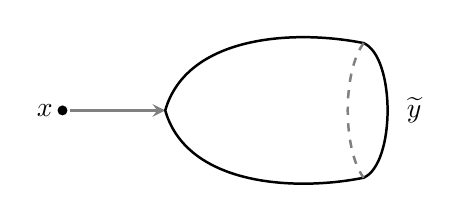
\begin{tikzpicture}[>=stealth,scale=.9]
  \fill (-3,0) circle (2pt) node[left] {$x$};
  \draw[->,gray,line width=1pt] (-2.9,0)--(-1.55,0);
  \draw[line width=.9pt] (-1.55,0)
    .. controls (-1.25,1.05) and (.25,1.15) .. (1.25,.95)
    .. controls (1.7,.75) and (1.7,-.75) .. (1.25,-.95)
    .. controls (.25,-1.15) and (-1.25,-1.05) .. (-1.55,0);
  \draw[gray,dashed,line width=.9pt] (1.25,.95)
    .. controls (.95,.55) and (.95,-.55) .. (1.25,-.95);
  \node[right] at (1.72,0) {$\widetilde y$};
\end{tikzpicture}
\caption{PSS 同构 $\Phi^\alpha:\operatorname{HF}^*\to\operatorname{QH}^*$。}
\label{fig:12-1-1}
\end{figure}

当 $\operatorname{ind}_f(x)-n=\mu_{\mathrm{CZ}}(\widetilde y)$ 时，\BookRecordIndex{T0182}尖盘\BookRecordIndex{T0246}模空间为零维，故可用
其元素数 $n(x,\widetilde y)$ 构造简称为 PSS 映射的链映射
\[
  \Phi^\alpha:\operatorname{CF}^*(H^\alpha)
  \longrightarrow\operatorname{CM}^*(f;\Lambda_\omega),
\]
定义为
\[
  (\Phi^\alpha\xi)(x,A):=
  \sum_{\mu_{\mathrm{CZ}}(\widetilde y)=\operatorname{ind}_f(x)-n}
  n(x,\widetilde y)\xi(A\#\widetilde y).
\]
这里 $\xi\in\operatorname{CF}^*(H^\alpha)$。为说明满足
$(\Phi^\alpha\xi)(x,A)\neq0$ 且 $\omega(A)\geq-c$ 的偶对 $(x,A)$ 只有有限多个，注意每个
这样的偶对都对应某个 $\widetilde y\in\widetilde{\mathcal P}(H^\alpha)$，使
$n(x,\widetilde y)\neq0$ 且 $\xi(A\#\widetilde y)\neq0$。后一不等式意味着存在常数
$c_\xi>0$，使 $\mathcal A_{H^\alpha}(A\#\widetilde y)\geq-c_\xi$；前一不等式意味着\BookRecordIndex{T0246}模空间
$\mathcal M(\widetilde y;H^\alpha,J^\alpha)$ 非空。因此由\BookRecordIndex{T0249}能量恒等式~\eqref{eq:12-1-11}，
存在只依赖 $(H^\alpha,J^\alpha)$ 的常数 $c_E>0$，使
\begin{equation}\label{eq:12-1-14}
  E(u)\leq c_E-\mathcal A_{H^\alpha}(\widetilde y)
  =c_E-\mathcal A_{H^\alpha}(A\#\widetilde y)-\omega(A)
  \leq c_E+c_\xi+c.
\end{equation}
这个一致能量界证明了所需有限性条件。

映射 $\Phi^\alpha$ 是把次数提高 $n$ 的 $\Lambda_\omega$-模同态。\BookRecordIndex{T0132}弗洛尔同调中的标准论证
（如 $\delta^2=0$ 的证明）说明它是链映射，因此在上同调上诱导仍记作 $\Phi^\alpha$ 的同态。
Piunikhin--Salamon--Schwarz \srcite{323} 证明了这个诱导同态是同构。其证明构造类似的
链映射
\[
  \Psi^\alpha:\operatorname{CM}^*(f;\Lambda_\omega)
  \longrightarrow\operatorname{CF}^*(H^\alpha),
\]
其公式为
\[
  (\Psi^\alpha\xi_0)(\widetilde x):=
  \sum_{\operatorname{ind}_f(y)-2c_1(A)=\mu_{\mathrm{CZ}}(\widetilde x)+n}
  n((-A)\#\widetilde x,y)\xi_0(y,A),
\]
其中 $\xi_0\in\operatorname{CM}^*(f;\Lambda_\omega)$。接下来须证明两个复合
$\Phi^\alpha\circ\Psi^\alpha$ 与 $\Psi^\alpha\circ\Phi^\alpha$ 都链同伦于恒等映射；
图~\ref{fig:12-1-2}、\ref{fig:12-1-3} 描绘了这一论证。技术核心是弗洛尔\BookRecordIndex{T0256}粘合定理以及
第~\ref{ch:gluing} 章证明的 \BookRecordIndex{T0003}$J$-全纯曲线\BookRecordIndex{T0256}粘合定理；如下方注~\ref{rem:12-1-7} 所述，
论证其余部分都是标准的。

\begin{figure}[tbp]
\centering
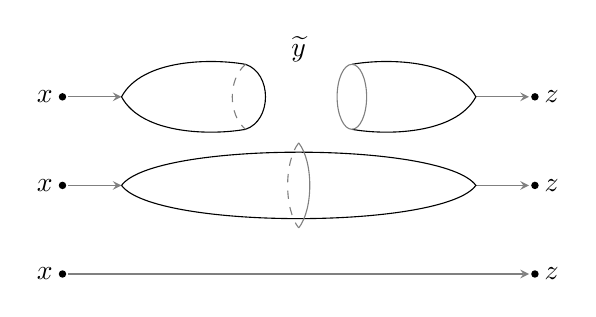
\begin{tikzpicture}[>=stealth,scale=.75]
  \foreach \y in {1.5,0,-1.5}{
    \fill (-4,\y) circle (1.8pt) node[left] {$x$};
    \fill (4,\y) circle (1.8pt) node[right] {$z$};
  }
  \draw[->,gray] (-3.9,1.5)--(-3,1.5);
  \draw[gray,->] (3,1.5)--(3.9,1.5);
  \draw (-3,1.5)
    .. controls (-2.65,2.15) and (-1.45,2.15) .. (-.9,2.05)
    .. controls (-.45,1.9) and (-.45,1.1) .. (-.9,.95)
    .. controls (-1.45,.85) and (-2.65,.85) .. (-3,1.5);
  \draw[gray,dashed] (-.9,2.05)
    .. controls (-1.2,1.8) and (-1.2,1.2) .. (-.9,.95);
  \draw (.9,2.05)
    .. controls (1.45,2.15) and (2.65,2.15) .. (3,1.5)
    .. controls (2.65,.85) and (1.45,.85) .. (.9,.95);
  \draw[gray] (.9,1.5) ellipse[x radius=.25,y radius=.55];
  \node at (0,2.3) {$\widetilde y$};
  \draw[->,gray] (-3.9,0)--(-3,0);
  \draw[gray,->] (3,0)--(3.9,0);
  \draw (-3,0)
    .. controls (-2.45,.75) and (2.45,.75) .. (3,0)
    .. controls (2.45,-.75) and (-2.45,-.75) .. (-3,0);
  \draw[gray,dashed] (0,.72)
    .. controls (-.25,.4) and (-.25,-.4) .. (0,-.72);
  \draw[gray] (0,.72)
    .. controls (.25,.4) and (.25,-.4) .. (0,-.72);
  \draw[->,gray] (-3.9,-1.5)--(3.9,-1.5);
\end{tikzpicture}
\caption{$\Phi^\alpha\circ\Psi^\alpha\simeq\operatorname{id}$。}
\label{fig:12-1-2}
\end{figure}

\begin{figure}[tbp]
\centering
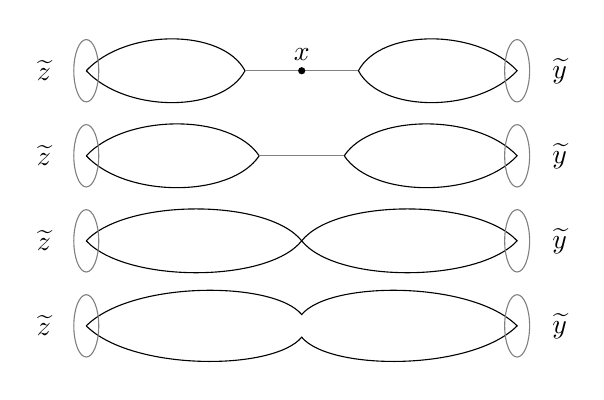
\begin{tikzpicture}[>=stealth,scale=.72]
  \foreach \y in {2.25,.75,-.75,-2.25}{
    \node[left] at (-4.25,\y) {$\widetilde z$};
    \node[right] at (4.25,\y) {$\widetilde y$};
  }
  \draw (-3.8,2.25) .. controls (-3.1,3) and (-1.4,3) .. (-1,2.25)
    .. controls (-1.4,1.5) and (-3.1,1.5) .. (-3.8,2.25);
  \draw (1,2.25) .. controls (1.4,3) and (3.1,3) .. (3.8,2.25)
    .. controls (3.1,1.5) and (1.4,1.5) .. (1,2.25);
  \draw[gray] (-1,2.25)--(1,2.25); \fill (0,2.25) circle (1.8pt) node[above] {$x$};
  \draw (-3.8,.75) .. controls (-3.1,1.5) and (-1.25,1.5) .. (-.75,.75)
    .. controls (-1.25,0) and (-3.1,0) .. (-3.8,.75);
  \draw (.75,.75) .. controls (1.25,1.5) and (3.1,1.5) .. (3.8,.75)
    .. controls (3.1,0) and (1.25,0) .. (.75,.75);
  \draw[gray] (-.75,.75)--(.75,.75);
  \draw (-3.8,-.75) .. controls (-3.1,0) and (-.6,0) .. (0,-.75)
    .. controls (-.6,-1.5) and (-3.1,-1.5) .. (-3.8,-.75);
  \draw (0,-.75) .. controls (.6,0) and (3.1,0) .. (3.8,-.75)
    .. controls (3.1,-1.5) and (.6,-1.5) .. (0,-.75);
  \draw (-3.8,-2.25) .. controls (-3,-1.45) and (-.5,-1.45) .. (0,-2.05)
    .. controls (.5,-1.45) and (3,-1.45) .. (3.8,-2.25)
    .. controls (3,-3.05) and (.5,-3.05) .. (0,-2.45)
    .. controls (-.5,-3.05) and (-3,-3.05) .. (-3.8,-2.25);
  \foreach \y in {2.25,.75,-.75,-2.25}{
    \draw[gray] (-3.8,\y) ellipse[x radius=.22,y radius=.55];
    \draw[gray] (3.8,\y) ellipse[x radius=.22,y radius=.55];
  }
\end{tikzpicture}
\caption{$\Psi^\alpha\circ\Phi^\alpha\simeq\operatorname{id}$。}
\label{fig:12-1-3}
\end{figure}

还要注意，若 $H=-f$ 与时间无关，并且处在弗洛尔原始论证适用的情形，那么可以证明：当
$\varepsilon>0$ 充分小时，对 PSS 映射有贡献的\BookRecordIndex{T0182}尖盘只有 $H$ 的\BookRecordIndex{T0233}临界点处的常值映射。因此
PSS 映射 $\operatorname{CF}^*(-\varepsilon f)\to\operatorname{CM}^*(f;\Lambda_\omega)$
就是显然的同构。由此，PSS 同构 $\Phi^\alpha$
\sourcefootnote{原书此处写作 $\Psi^\alpha$，但本段比较的是从弗洛尔上同调到\BookRecordIndex{T0229}量子上同调的
PSS 映射；按定理~\ref{thm:12-1-4} 及紧邻公式，该方向记为 $\Phi^\alpha$。}
在弗洛尔方法所构造的映射有定义时，与后者相同。

\begin{remark}\label{rem:12-1-7}
可以把 PSS 映射
\[
  \Phi^*_{\mathrm{PSS}}:\operatorname{CF}^*(H^\alpha)
  \longrightarrow\operatorname{CM}^*(f;\Lambda_\omega)
\]
看作 Seidel 同态 $\mathcal S(\phi)$ 的“一半”。如注~\ref{rem:11-4-4} 所述，Seidel 同态
通过计数 $S^2$ 上某个丛的截面给出，这些截面与位于两个固定点 $w_1,w_2$ 上纤维中的循环
相交。若用某个 Morse 流的不稳定流形表示 $w_1$ 上纤维中的循环，以稳定流形表示 $w_2$
上纤维中的循环，那么所计数的是带两个尖部的球面：一个尖部是从 $x$ 出发的梯度轨道，
另一个是流向 $z$ 的梯度轨道；参见图~\ref{fig:12-1-2}。在当前情形，计数的是带弗洛尔
边界条件的圆盘上截面。沿边界把两个定向相反的这种圆盘\BookRecordIndex{T0254}粘合，就得到 Seidel 所计数的一个
球面。

因此，$\Phi^*_{\mathrm{PSS}}\circ\Psi^*_{\mathrm{PSS}}$ 是\BookRecordIndex{T0229}量子上同调上的恒等映射这一
断言，等价于定义~\ref{def:11-4-1} 的 \BookRecordIndex{T0046}Seidel 元 $\mathcal S(\operatorname{id},\sigma_0)$
是 $\operatorname{QH}^0(M;\Lambda)$ 中的幺元。（这里 $\operatorname{id}$ 是群
$\pi_1(\operatorname{Ham}(M))$ 的单位元，$\sigma_0$ 表示 $S^2\times M$ 中的平凡\BookRecordIndex{T0189}截面类
$[S^2\times\{\mathrm{pt}\}]$。）在当前背景以及 Piunikhin--Salamon--Schwarz
\srcite{323} 的背景中，\BookRecordIndex{T0254}粘合在拓扑上平凡，产生平凡丛的一个截面。Seidel \srcite{363}
指出，这些思想可以调整后用于非平凡丛；见第~\ref{sec:12-5} 节。Lalonde \srcite{222} 进一步发展了
这一观点。
\end{remark}
